% !TeX root = ../main.tex


\section{Ejercicio 1: Requisitos}\label{sec:ejercicio-1:-requisitos}
% !TeX root = ../examen-parcial-2023.tex


\begin{itemize}
    \item \textbf{Puntos:} 2
\end{itemize}
\begin{enunciado}
    El actual equipo de desarrollo está aplicando las siguientes prácticas:
    \begin{enumerate}
        \item El equipo planifica entregas trimestrales que incluyen un conjunto de funcionalidades acordadas entre el director de ingeniería y el director de producción dentro un plan anual.
        \item El equipo se asegura que el conjunto de funcionalidades de las entregas trimestrales se comporta correctamente y es usado por los usuarios finales sin dificultades.
        \item El equipo se comunica directamente con el director de producción cuando tiene dudas acerca de cómo debe comportarse una funcionalidad concreta.
        \item Dentro del equipo cada miembro tiene su función: una persona diseña la solución, otro la construye, otro la prueba y otro la despliega y mantiene en producción.
    \end{enumerate}
    Lee detenidamente las prácticas e:
    \begin{enumerate}
        \item Identifica, para cada una de ellas, si se corresponden con prácticas ágiles.
        \item Justifica las respuestas en base al manifiesto ágil.
        \item \textbf{0,3 cada respuesta correcta con justificación.}
        \item Indica qué cambios aplicarías en las que no son ágiles (si hay alguna) para que sí lo sean.
        \item \textbf{0,4 por cada práctica convertida en ágil.}
    \end{enumerate}
\end{enunciado}

\begin{solucion}
    \begin{enumerate}
        \item \textbf{Práctica 1:} NO ágil.
        Se incumple el valor Respuesta ante el cambio sobre seguir un plan.
        \begin{itemize}
            \item \textbf{Cambios para que fuera ágil:}
            \begin{itemize}
                \item Ciclos de desarrollo más cortos (2 a 4 semanas).
                \item Identificación y priorización de funcionalidades en cada ciclo.
            \end{itemize}
        \end{itemize}

        \item \textbf{Práctica 2:} Ágil.
        Se cumple el valor Software funcionando sobre documentación extensiva.

        \item \textbf{Práctica 3:} Ágil.
        Se cumple el valor Colaboración con el cliente sobre negociación contractual.

        \item \textbf{Práctica 4:} NO ágil.
        Se incumple el valor Individuos e interacciones sobre procesos y herramientas.
        \begin{itemize}
            \item \textbf{Cambios para que fuera ágil:}
            \begin{itemize}
                \item Individuos multidisciplinares.
                \item Colaboración entre los miembros para realizar las diferentes funciones.
            \end{itemize}
        \end{itemize}
    \end{enumerate}
\end{solucion}



\section{Ejercicio 2: Casos de uso e historias de usuario}\label{sec:ejercicio-2:-casos-de-uso-e-historias-de-usuario}
% !TeX root = ../examen-parcial-2023.tex

\begin{itemize}
    \item \textbf{Puntos:} 3
\end{itemize}

\begin{enunciado}
    Se han identificado los siguientes requisitos como parte de la mejora de la gestión de la
    producción:
    \begin{enumerate}
        \item Los gestores deben poder acceder al sistema a través de una interfaz web mientras que
        los agricultores deben poder hacerlo mediante una aplicación móvil disponible para iOS\@.
        \item Los gestores de producción deben poder añadir y eliminar campos de cultivo al sistema.
        \item Los agricultores deben poder registrar las labores realizadas en los campos de cultivo
        (arado, siembra, riego, abonado, recolección, etc.) mediante geolocalización.
        \item Los agricultores deben poder notificar incidencias que afecten a la producción (plagas,
        eventos climatológicos, etc.).
        \item El equipo de desarrollo debe poder saber si el sistema está funcionando correctamente.
        \item Los gestores deben poder anotar la producción recolectada en cada campo.
        \item La aplicación debe tener un porcentaje de disponibilidad anual del 99.99\%.
        \item Los gestores deben poder marcar el estado de un campo (barbecho, activo, etc.).
    \end{enumerate}
    Lee detenidamente los requisitos y:
    \begin{enumerate}
        \item Clasifica los requisitos en funcionales, no funcionales u otros.
        \item $0.2$ puntos por cada respuesta correcta.
        \item Desarrolla la especificación del caso de uso de uno de los requisitos que hayas
        clasificado como funcional.
        \item $0.2$ puntos por cada campo simple; $0.3$ puntos por cada campo
    \end{enumerate}
\end{enunciado}
\begin{solucion}
    \begin{enumerate}
        \item Clasificación de los requisitos:
        \begin{itemize}
            \item Requisito 1: No funcional.
            \item Requisito 2: Funcional.
            \item Requisito 3: Funcional.
            \item Requisito 4: Funcional.
            \item Requisito 5: Otros.
            \item Requisito 6: Funcional.
            \item Requisito 7: No funcional.
            \item Requisito 8: Funcional.
        \end{itemize}

        \item Especificación del caso de uso (ejemplo para el requisito 2):
        \begin{itemize}
            \item Nombre: Añadir campo de cultivo.
            \item Actor: Gestor de producción.
            \item Descripción: Los gestores de producción deben poder añadir y eliminar campos de cultivo al sistema.
            \item Precondiciones: El gestor de producción debe haber iniciado sesión en el sistema.
            \item Dependencias: No especificado.
            \item Escenario:
            \begin{enumerate}
                \item El gestor de campo comienza el proceso de añadir un campo.
                \item El gestor de campo rellena los detalles del campo (nombre, localización,\ldots ).
                \item El gestor graba el campo en el sistema.
            \end{enumerate}
            \item Excepciones:
            \begin{enumerate}
                \item El gestor de campo comienza el proceso de añadir un campo.
                \item El gestor de campo no rellena todos los detalles del campo.
                \item El gestor de campo intenta grabar el campo en el sistema.
                \item El sistema indica que faltan detalles del campo.
            \end{enumerate}
        \end{itemize}
    \end{enumerate}
    \begin{itemize}
        \item Prioridad: No especificado.
    \end{itemize}
\end{solucion}


\section{Ejercicio 3: Diagrama de secuencia}\label{sec:ejercicio-3:-diagrama-de-secuencia}
% !TeX root = ../examen-parcial-2023.tex
%
%Analiza detenidamente el diagrama y:
%A) Asocia los componentes con los requisitos que cubren. - 0,4 por cada requisito
%Interfaz web e interfaz móvil. Requisito 1.
%Gestor de campos. Requisitos 2 y 8.
%Registrador de labores. Requisito 3.
%Administrador de incidencias. Requisito 4.
%B) Completa el diagrama con los componentes necesarios para cubrir todos los requisitos
%funcionales del Ejercicio 2. - 1 punto
%Gestor de producción. Conectado al canal de comunicación. Requisito 6.

\begin{itemize}
    \item \textbf{Puntos:} 3
\end{itemize}

\begin{enunciado}
    El equipo de desarrollo ha realizado esta primera versión del diagrama de arquitectura para
    cubrir los requisitos funcionales del Ejercicio 2:


    \deactivatequoting

    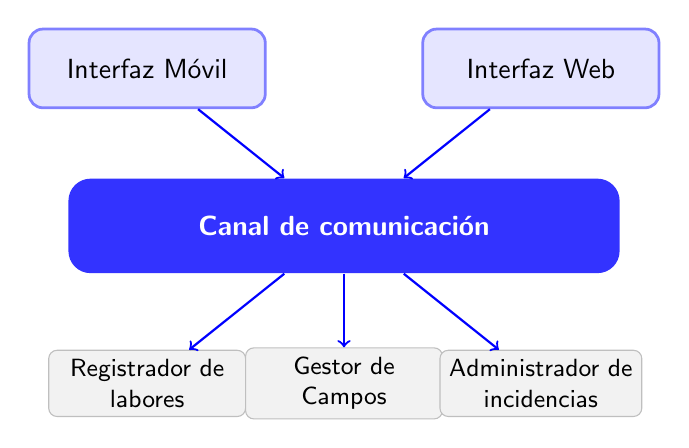
\begin{tikzpicture}[
    % Estilos máis simples pero modernos
        interface/.style={
            rectangle,
            rounded corners=5pt,
            fill=blue!10,
            draw=blue!50,
            line width=1pt,
            font=\sffamily,
            minimum width=3cm,
            minimum height=1cm,
            align=center
        },
        communication/.style={
            rectangle,
            rounded corners=8pt,
            fill=blue!80,
            text=white,
            font=\sffamily\bfseries,
            minimum width=7cm,
            minimum height=1.2cm,
            align=center
        },
        component/.style={
            rectangle,
            rounded corners=3pt,
            fill=gray!10,
            draw=gray!50,
            font=\sffamily\small,
            minimum width=2.5cm,
            minimum height=0.8cm,
            align=center
        }
    ]

        % Interfaces superiores
        \node[interface] (interfaz_movil) at (0, 3) {Interfaz Móvil};
        \node[interface] (interfaz_web) at (5, 3) {Interfaz Web};

        % Canal de comunicación
        \node[communication] (canal) at (2.5, 1) {Canal de comunicación};

        % Compoñentes inferiores
        \node[component] (registrador) at (0, -1) {Registrador de\\labores};
        \node[component] (gestor) at (2.5, -1) {Gestor de\\Campos};
        \node[component] (administrador) at (5, -1) {Administrador de\\incidencias};

        % Conexiones
        \draw[->, thick, blue] (interfaz_movil) -- (canal);
        \draw[->, thick, blue] (interfaz_web) -- (canal);
        \draw[->, thick, blue] (canal) -- (registrador);
        \draw[->, thick, blue] (canal) -- (gestor);
        \draw[->, thick, blue] (canal) -- (administrador);

    \end{tikzpicture}

    \begin{enumerate}
        \item Analiza detenidamente el diagrama y:
        \begin{enumerate}
            \item Asocia los componentes con los requisitos que cubren.
            \item Completa el diagrama con los componentes necesarios para cubrir todos los requisitos
            funcionales del Ejercicio 2.
        \end{enumerate}
        \item \textbf{0,4 puntos por cada requisito asociado.}
        \item \textbf{1 punto por completar el diagrama.}
    \end{enumerate}

\end{enunciado}

\begin{solucion}
    \begin{enumerate}
        \item Análisis del diagrama:
        \begin{enumerate}
            \item Asociaciones de componentes con requisitos:
            \begin{itemize}
                \item Interfaz web e interfaz móvil: Requisito 1.
                \item Gestor de campos: Requisitos 2 y 8.
                \item Registrador de labores: Requisito 3.
                \item Administrador de incidencias: Requisito 4.
            \end{itemize}

            \item Componentes necesarios para cubrir todos los requisitos funcionales:
            \begin{itemize}
                \item Gestor de producción: Conectado al canal de comunicación: Requisito 6.
            \end{itemize}
        \end{enumerate}
    \end{enumerate}
\end{solucion}


\section{Ejercicio 5: Tiempo medio entre fallos y tiempo de recuperación}\label{sec:ejercicio-5:-tiempo-medio-entre-fallos-y-tiempo-de-recuperacion}
% !TeX root = ../planificacion.tex

\begin{enunciado}
    Desarrolla el diagrama de PERT del conjunto de tareas del ejercicio 3.
    ¿Qué tareas están en el camino crítico?
\end{enunciado}

\begin{solucion}

    La duración total del proyecto es de \textbf{33 días}, determinada por el camino crítico:

    A → C → E → F → G → H → I → J\@.

    Diagrama PERT de las \textbf{tareas del ejercicio 3}:

    \deactivatequoting
    \tikz[>={To[sep]}, rotate=90, xscale=-1]
    \graph [nodes={circle,draw},
        edges={nodes={inner sep=1pt, anchor=mid}}]
    {
        A ->
            {
                {
                B ->
                    {
                    D
                }
            }
            ,
                {
                C ->
                    {
                    E ->
                        {
                        F
                    }
                }
            }
        } ->
            {
            G ->
                {
                H ->
                    {
                    I ->
                        {
                        J
                    }
                }
            }
        }
    };
    \activatequoting
\end{solucion}


\clearpage


\section{Ejercicio 6: Requisitos}\label{sec:ejercicio-6-:-requisitos}
% !TeX root = ../modelado.tex


\begin{enunciado}
    Clasifica los siguientes requisitos no funcionales en su correspondiente subcategoría:
    \begin{enumerate}
        \item La aplicación debe funcionar en Windows, Unix, MacOs, Android e iOS
        \item La aplicación debe usar lenguaje inclusivo
        \item La aplicación debe estar disponible de lunes a viernes de 8h a 18h
        \item La operación de registro debe realizarse en menos de 1 segundo
        \item La versión móvil de la aplicación debe ocupar menos de 100MB
        \item La aplicación debe ser compatible con el sistema de videoconferencia Zoom
        \item Se deben entregar tanto los ejecutables de las diferentes versiones como el código fuente
        \item La aplicación debe ser accesible para personas con discapacidades visuales o motoras.
    \end{enumerate}
\end{enunciado}

\begin{solucion}
    \begin{enumerate}
        \item De proceso, implementación, usabilidad
        \item Externos, legislativo, seguridad
        \item Producto, usabilidad
        \item Producto, eficiencia, espacio
        \item Producto, usabilidad, implementación
        \item Proceso, delivery
        \item Ética?
    \end{enumerate}
\end{solucion}


\clearpage


\section{Ejercicio 7: Diagrama de arquitectura}\label{sec:ejercicio-7:-diagrama-de-arquitectura}
% !TeX root = ../modelado.tex

\begin{enunciado}
    Completa el diagrama de arquitectura para añadir la siguiente funcionalidad:

    Aplicación de ofertas en función de la cantidad de productos comprados y el país desde el
    que se realiza la compra.
\end{enunciado}


\begin{solucion}

    \begin{tikzpicture}[node distance=1.25cm]
% Interfaz Gráfica
        \hspace{1em}
        \node[interface] (gui) {Interfaz Gráfica};

% Primera fila de servicios
        \node[service, below left=2cm and 1.5cm of gui] (catalog) {CatalogService};
        \node[service, below=2cm of gui] (cart) {CartService};
        \node[service, below right=2cm and 1.5cm of gui] (order) {OrderService};

% Segunda fila de servicios
        \node[service, below =2.0cm of catalog] (pricing) {PricingService};
        \node[service, below =2cm of order] (payment) {PaymentService};

% Nuevo servicio de ofertas (añadido)
        \node[service, below=2.0cm of cart, fill=green!20] (offers) {OffersService};

% Servicio de geolocalización (añadido)
        \node[service, below left=1.5cm and -0.5cm of offers, fill=orange!20] (geo) {GeoService};

% Bases de datos
        \node[database, left=0.5cm of catalog] (db1) {};
        \node[database, above= 0.25cm of cart,xshift=0.5cm] (db2) {};
        \node[database, right=0.5cm of order] (db3) {};
        \node[database, left=0.5cm of pricing] (db4) {};
        \node[database, right=0.5cm of offers] (db6) {};
        \node[database, left=0.5cm of geo] (db7) {};

% Conexiones desde la interfaz
        \draw[arrow] (gui) -- (catalog);
        \draw[arrow] (gui) -- (cart);
        \draw[arrow] (gui) -- (order);

% Conexiones entre servicios
        \draw[bidirectional] (catalog) -- (cart);
        \draw[bidirectional] (cart) -- (order);
        \draw[bidirectional] (catalog) -- (pricing);
        \draw[bidirectional] (order) -- (payment);

% Nuevas conexiones para ofertas
        \draw[bidirectional] (cart) -- (offers);
        \draw[bidirectional] (order) -- (offers);
        \draw[bidirectional] (offers) -- (geo);
        \draw[bidirectional] (offers) -- (pricing);

% Conexiones a bases de datos
        \draw[arrow] (catalog) -- (db1);
        \draw[arrow] (cart) -- (db2);
        \draw[arrow] (order) -- (db3);
        \draw[arrow] (pricing) -- (db4);
        \draw[arrow] (offers) -- (db6);
        \draw[arrow] (geo) -- (db7);

% Etiquetas para las nuevas funcionalidades
        \node[above=0.2cm of offers, font=\tiny, text=green!60!black] {Gestión de ofertas};
        \node[above=0.2cm of geo, font=\tiny, text=orange!60!black] {Geolocalización};

    \end{tikzpicture}

\end{solucion}


\section{Ejercicio 8: Interfaz textual}\label{sec:ejercicio-8:-interfaz-textual}
% !TeX root = ../modelado.tex


\begin{enunciado}
    Diseña una interfaz textual para las siguientes funcionalidades:

    \begin{itemize}
        \item Registrar películas vistas con su título y fecha de visualización
        \item Listar las películas vistas permitiendo ordenarlas por título o por fecha de visualización
    \end{itemize}
\end{enunciado}

\begin{solucion}
    Componente visual, imagen de la portada de la película


    Componente caja de texto para introducir el texto


    Componente campo de texto para introducir la fecha


    Búsqueda de datos para almacenar películas


    Componente visual para elegir si mostrar por fecha o por titulo
\end{solucion}